\begin{frame}{Results}{Angle Range}

  \begin{block}{Goal}
	Describing the movement of the antennas when the UA is flying far away from the GS. 
  \end{block}

  \begin{figure}[H]
    \centerline{
    \subfigure[UAS Map]{
    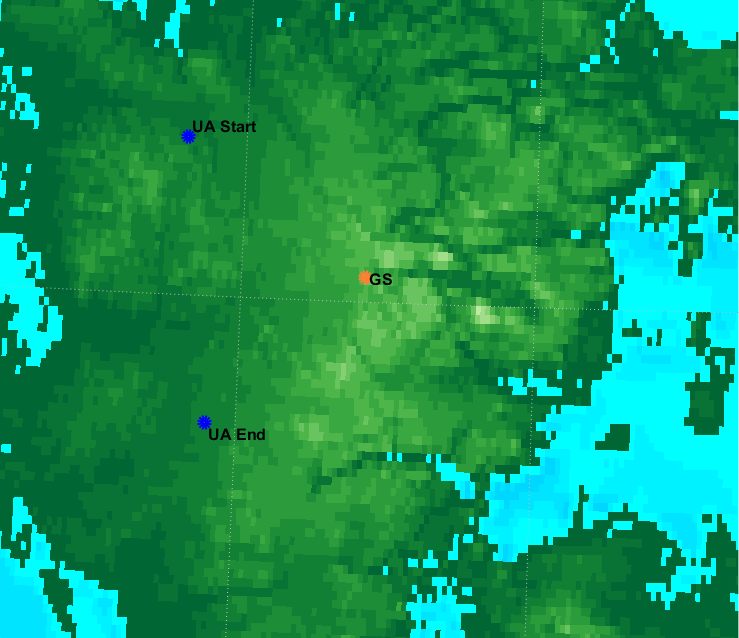
\includegraphics[scale=0.3]{figures/s1_zoom.png}}
    \subfigure[Distance between UA and GS]{
    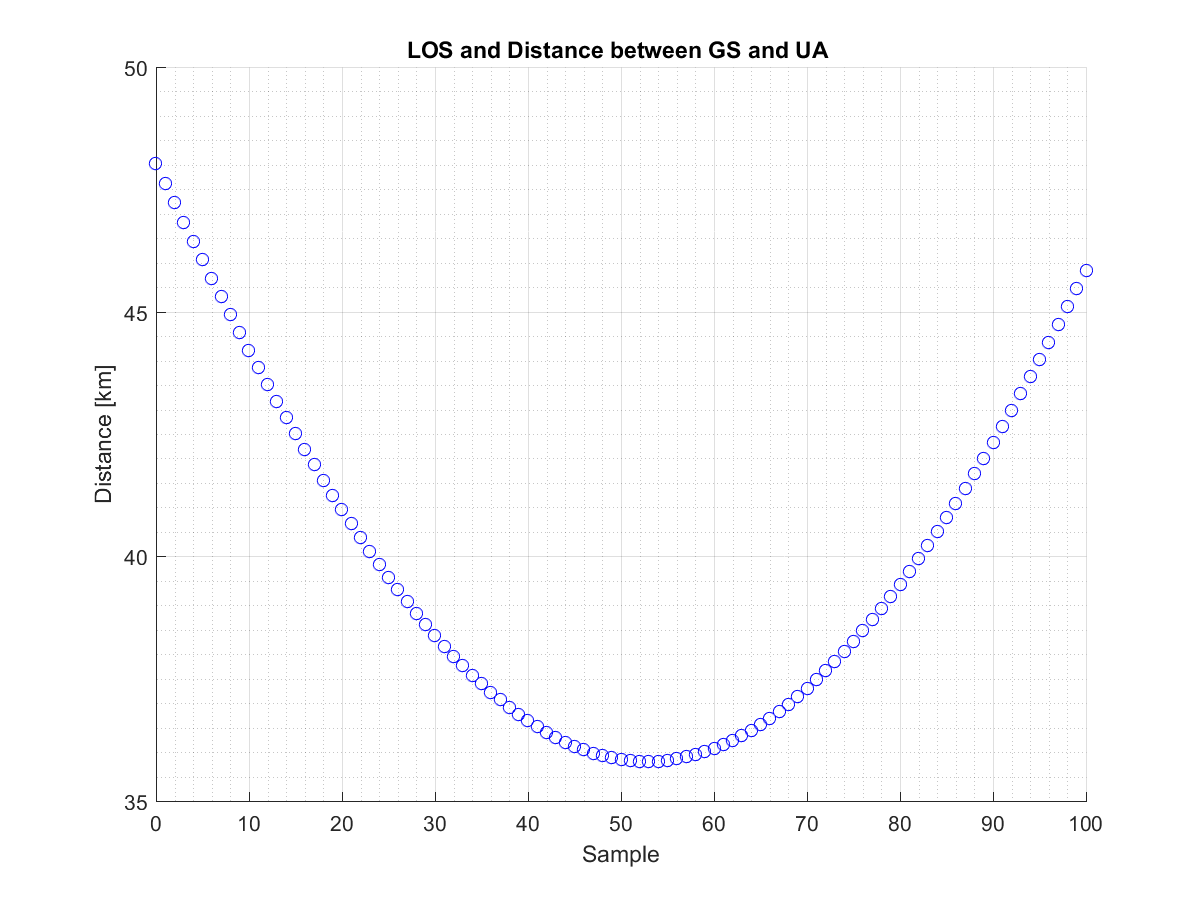
\includegraphics[scale=0.31]{figures/s1_los.png}}}
  \end{figure}

\end{frame}



\begin{frame}{Results}{Angle Range}

  \begin{block}{GS Tracking Angles}  
  
  \begin{figure}[H]
    \centerline{
    \subfigure[UAS Map]{
    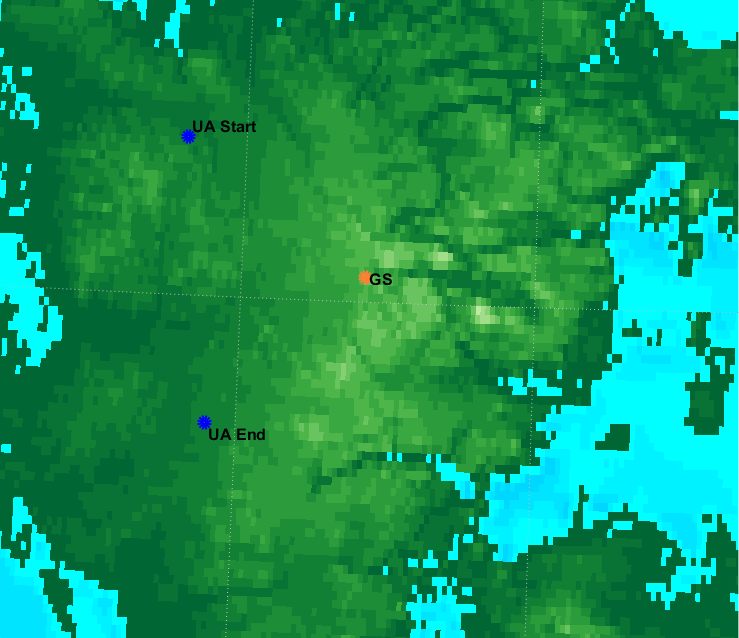
\includegraphics[scale=0.25]{figures/s1_zoom.png}}
    \subfigure[Distance between UA and GS]{
    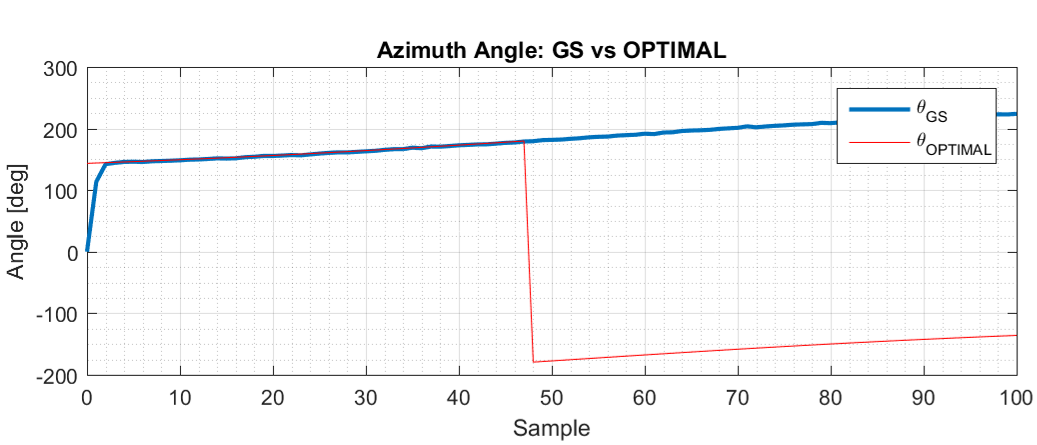
\includegraphics[scale=0.35]{figures/s1_pd_gs.png}}}
  \end{figure}
  
  \end{block}

\end{frame}